\begin{figure}[ht]
    % COMPLETE DIAGRAM
    \begin{subfigure}{0.6\textwidth}
    \centering
    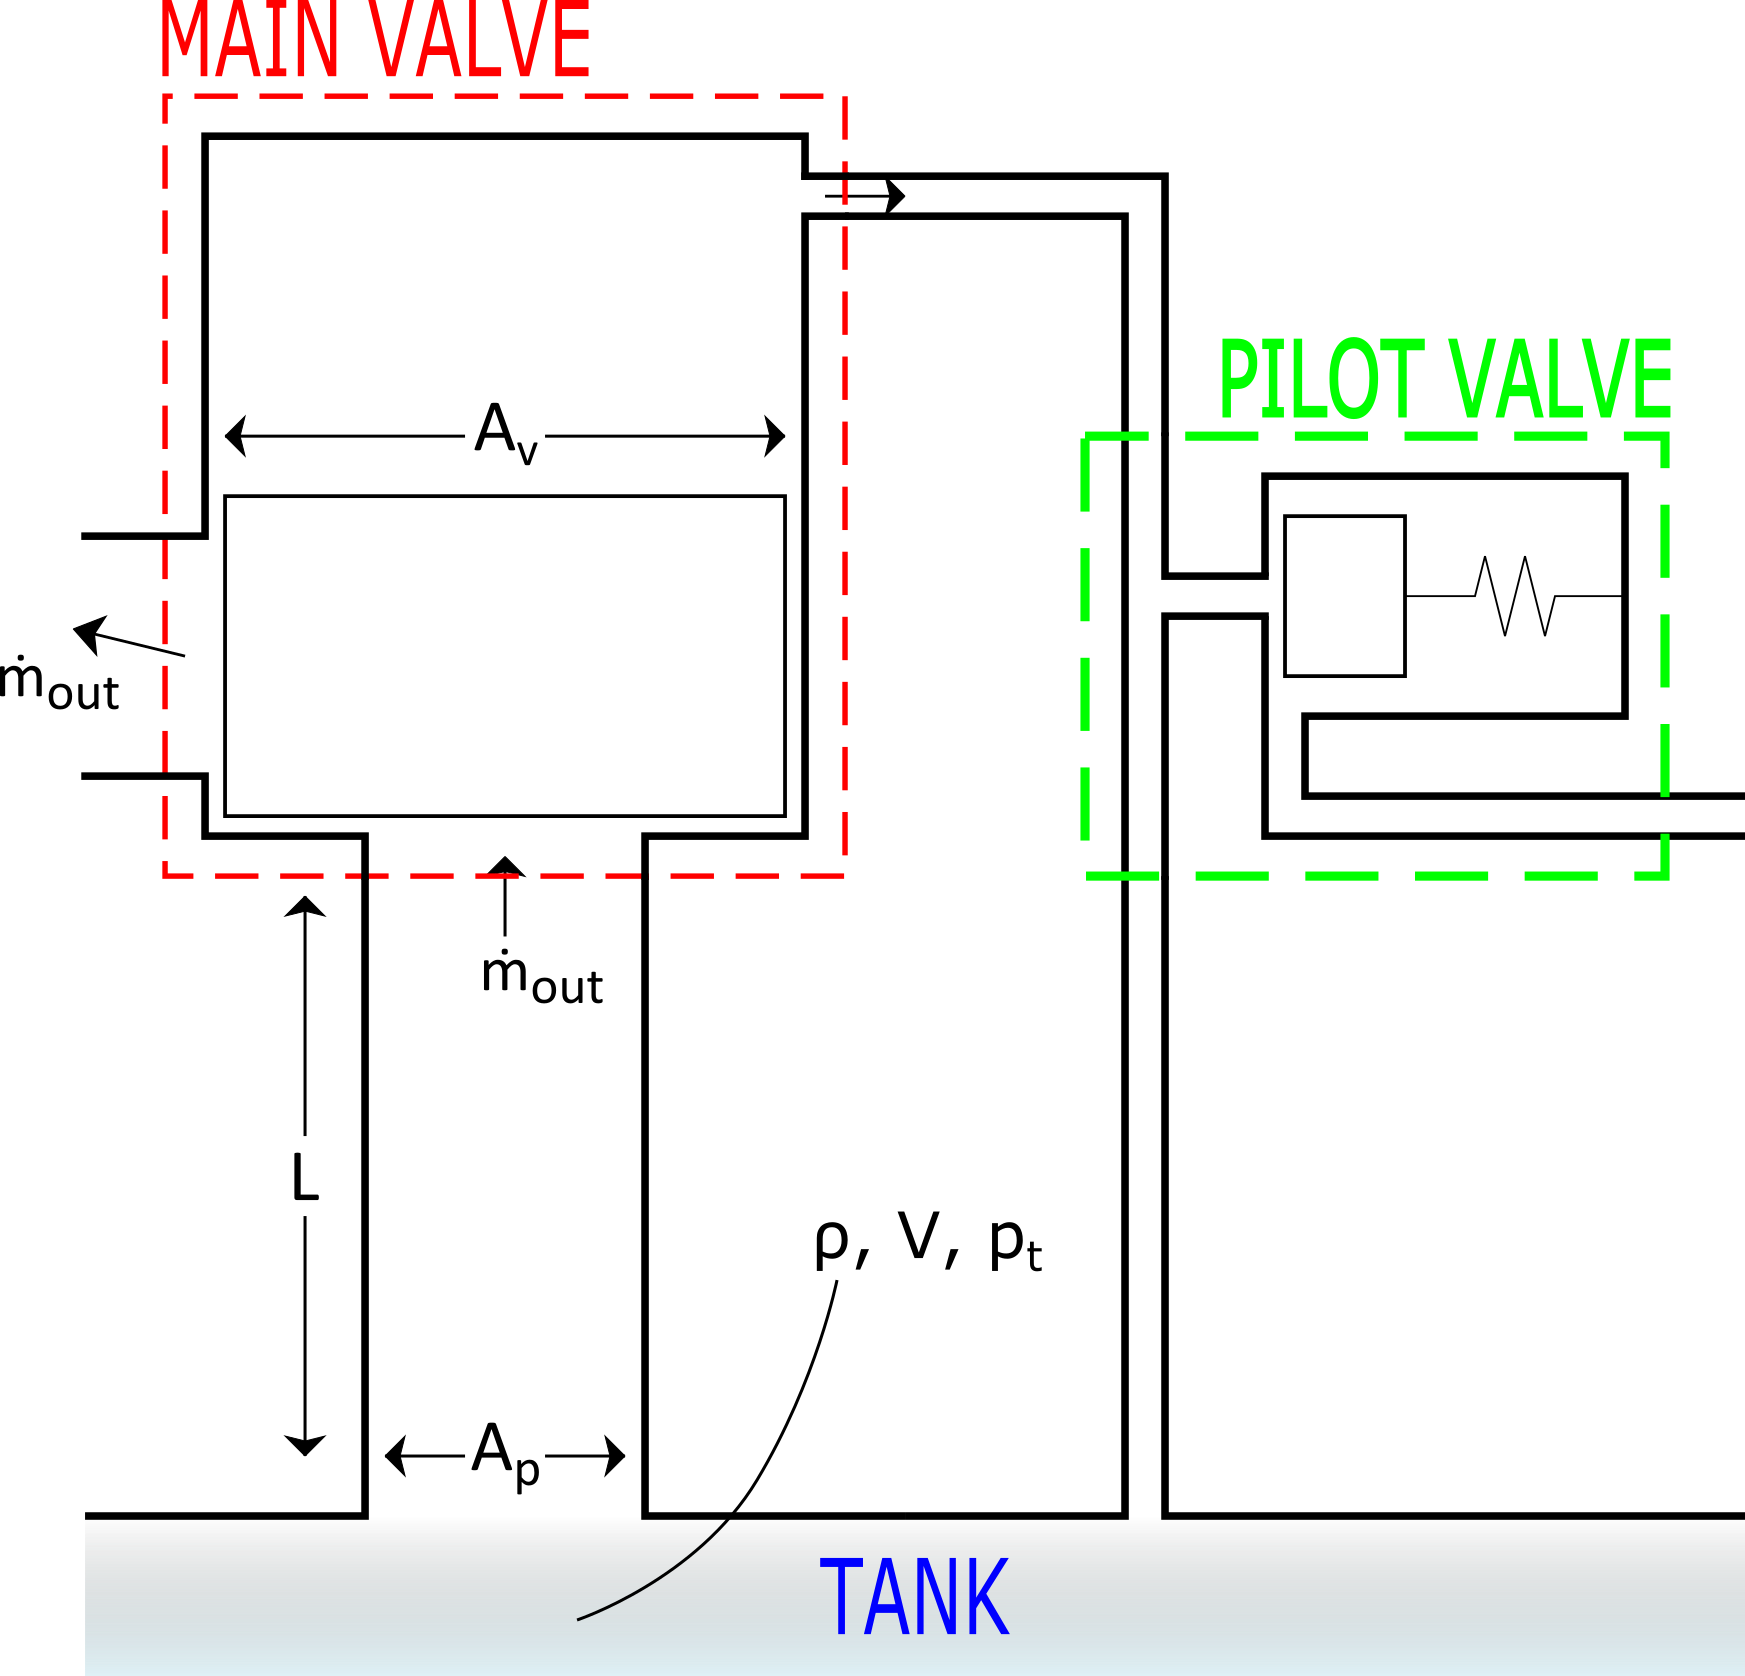
\includegraphics[width=\textwidth]{Diagrams/Diagram.png}
    \caption{Complete valve}
    \label{fig: DiagramComp}
    \end{subfigure}
    \hfill
    % Separate valve figures
    \begin{minipage}{0.3\textwidth}
        % MAIN DIAGRAM
        \begin{subfigure}{\textwidth}
        \centering
        
\includegraphics[width=\textwidth]{Diagrams/Diagram-Main.png}
        \caption{Main Valve}
        \label{fig: DiagramMain}
        \end{subfigure}
        % PILOT DIAGRAM
        \begin{subfigure}{\textwidth}
        \centering
        
\includegraphics[width=\textwidth]{Diagrams/Diagram-Pilot.png}
        \caption{Pilot Valve}
        \label{fig: DiagramPilot}
        \end{subfigure}
    \end{minipage}
    % Figure caption and label
    \caption{Diagram of pilot-operated pressure relief valve}
    \label{fig: Diagram}
\end{figure}